\chapter{Introduction}
\label{ch:introduction}
\graphicspath{{mainmatter/introduction/figures/}}

Within the last half-decade, we have seen an explosion of cloud-based services typically marketed under an \gls{ai} banner. 
Vendors are rapidly pushing out \gls{ai}-based solutions, technologies and products that encapsulate half a century worth of machine-learning research: a \citeyear{LoGiudice:2016wf} report by market research company Forrester captured such growth into four key areas \citep{LoGiudice:2016wf} as replicated in  \cref{fig:introduction:ai-products}. 
Application developers are eager to develop the next generation of `\gls{ai}-first' software, that will reason, sense, think, act, listen, speak and execute every whim in our web browser or smartphone app.
%A wave of \gls{ai}-first thinking embedded in companies' product lines is spearheaded through work achieved at Google, Microsoft and Facebook; for instance, Google's 2018 rebranding of \textit{Google Research} to \textit{Google AI} \citepweb{Howard:2018tz} or how \gls{ai} is leveraged \textit{at scale} within Facebook's infrastructure and platforms to serve its users with an \gls{ai}-first attitude \citep{Parekh:2017hx}.
%These services aim to lower the entry barrier to develop, test and deploy \gls{ai}-first software in both skill and time. 
%Application developers needn't require a formal training in \gls{ml} nor a strong understanding of mathematics: thus, \textit{skill required} is reduced. The training of such classifiers involves the laborious process of sourcing, curating and labelling large datasets: using such services does not, and thus \textit{time} is reduced. The process is abstracted behind an \glsac{api} call, only requiring knowledge on how to use a \glsac{rest}ful architecture \citep{Fielding:2000vh} (or similar) to access the cloud-based service.

A contrast is how these systems shift away from the traditional software engineering paradigm that application developers are comfortable with. Typical systems built by application developers are \textit{rule-driven} (or algorithm-driven), deterministically human engineered using source code to drive each step behind the application. These rule-driven systems typically consume, utilise, and integrate libraries and frameworks, \glsacpl{ide} and other tooling, and cloud-based services such as \gls{aws} \citep{AWS:Home}. The \gls{ai}-first software is, however, not rule-driven but \textit{data-driven}, fuelled with large datasets used to train \gls{ml} prediction algorithms and classifiers that present a typically probabilistic and nondeterministic behaviour.

So, how does the application developer approach her \gls{ai}-first application? To answer this, let us consider three approaches that could be used:

\begin{enumerate}
  \item She writes her own \gls{ml} classifier from scratch and trains it from her own curated dataset. This approach is laborious in time and demands formal training in \gls{ml} and mathematical knowledge, but the tradeoff is that she has full autonomy over the models she creates.
  \item She downloads a pre-trained model and `plugs' it into an existing \gls{ml} framework, such as Tensorflow \citep{Abadi:2016vn}. While this approach is less demanding in time, it still requires her to revise and understand the `glue' of the \gls{ml} framework code\footnote{Thus introducing a verbose list of \gls{ml} terminology to her already-required developer vocabulary. See a list of 328 terms provided by Google here: \url{https://developers.google.com/machine-learning/glossary/}.} with her own application code.
  \item She uploads her data to a pre-existing cloud-based service: a \textit{`Friendly' \acrlong{ml}} service. She doesn't need to know anything behind the underlying `intelligence' and how it works, is fast to integrate into her application and all abstracted behind a web-based \gls{api} call.
\end{enumerate}

\noindent
At first sight, she perceives the data-driven cloud service as `just another' cloud service  offered in her toolchain. Her perception is that just because this is another cloud service, it should act and behave as any other typical service would. But internally, she isn't aware that it this particular cloud service isn't a typical one; the data-driven service does not adapt to her rule-driven application in the way that she thinks (\cref{fig:introduction:rule-vs-data}). This is because the nature of typical cloud systems and data-driven ones are not exactly the same (\cref{tab:introduction:characteristics-of-cloud}).

\begin{figure}[h!]
\centering
\caption[Differences between data- and rule-driven cloud services]{The application developer's rule-driven toolchain is distinct from data-driven toolchain. A developer must consume a typical, data-driven cloud service in a different way than an intelligent data-driven cloud service as they are not the same type of system.}
\label{fig:introduction:rule-vs-data}
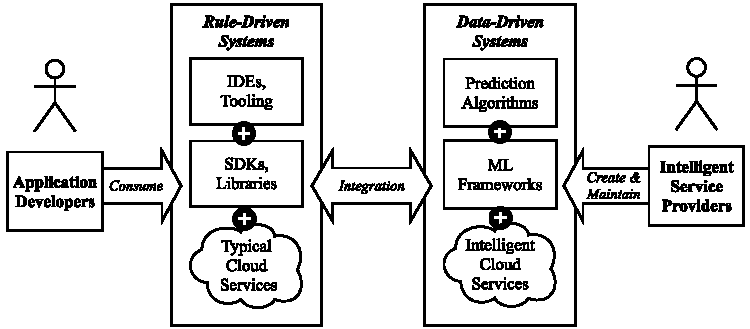
\includegraphics{rule-vs-data}
\end{figure}

\begin{table}[p]
\centering
\caption[Differing characteristics of cloud services]{Differing characteristics of intelligent and typical cloud services.}
\label{tab:introduction:characteristics-of-cloud}
\begin{tabular}{@{}ll@{}}
\toprule
  % Heading
  \textbf{Intelligent Cloud Services} &
  \textbf{Typical Cloud Services}
  \\
  \midrule
  Probabilistic &
  Deterministic 
  \\
  Machine Learnt &
  Human Engineered
  \\
  Data-Driven &
  Rule-Driven
  \\
  Black-Box &
  Mostly Transparent
  \\
  \bottomrule
\end{tabular}
\end{table}


This `range' of \gls{ai}-first integration techniques partially reflects Google AI's\footnote{
Google AI was recently rebranded from Google Research, further highlighting how the `\gls{ai}-first' philosophy is increasingly becoming embedded in companies' product lines and research and development teams. Spearheaded through work achieved at Google, Microsoft and Facebook, the emphasis can be seen through Google's 2018 rebranding of \textit{Google Research} to \textit{Google AI} \citepweb{Howard:2018tz} or how \gls{ai} is leveraged \textit{at scale} within Facebook's infrastructure and platforms to serve its users with an \gls{ai}-first attitude \citep{Parekh:2017hx}.
} 
\textit{\acrlong{ml} Spectrum} \citep{Ortiz:2017wg,LaForge:2018tm,McGowen:2019vt}, which encompasses the variety of skill, effort, users and types of outputs of integration techniques. On one extreme is the research of developing algorithms to achieve intelligence, produced chiefly in academia---coined as \gls{byoml} \citep{Ortiz:2017wg,McGowen:2019vt,Jimerson:2017vh}. On the other, such intelligence becomes heavily abstracted as easy-to-use \glspl{api}, targeted mainly towards developers as `friendly' \gls{ml}. In the middle lies a broad mix of combining both cloud and locally-hosted solutions (with varying levels of automation to assist in development) that turn custom datasets into some form of predictive intelligence. 

All techniques in this spectrum are data-driven, and we illustrate their slightly varied characteristics further in \cref{tab:introduction:comparison-of-ml-spectrum} and examples of the computer vision spectrum in \cref{fig:introduction:cv-spectrum}.

\begin{figure}[h!]
\centering
\caption[The spectrum of machine learning]{Examples within the machine learning spectrum of computer vision. Benefits and drawbacks of each end of the spectrum are indicated with the colour scales.}
\label{fig:introduction:cv-spectrum}
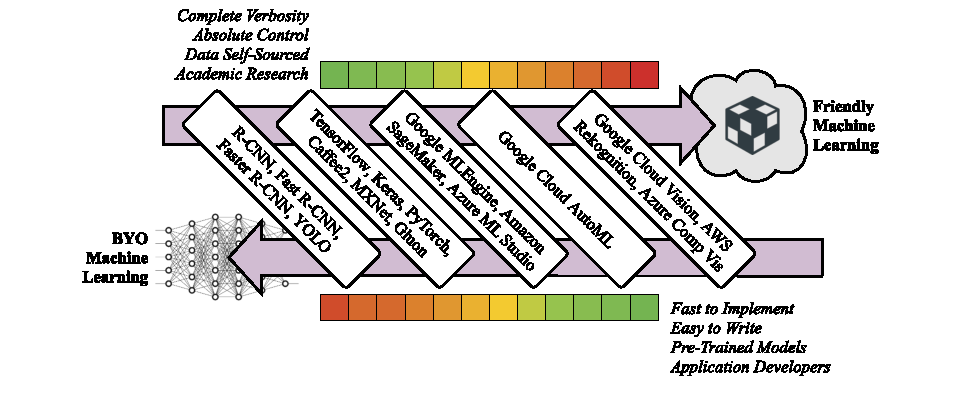
\includegraphics[width=\linewidth]{cv-spectrum}
\end{figure}

\begin{table}[p]
\centering
\caption[Comparison of the machine learning spectrum]{Comparison of the machine learning spectrum.}
\label{tab:introduction:comparison-of-ml-spectrum}
\begin{tabular}{@{}l|ccccc@{}}
\toprule
  % Heading
  \textbf{Comparator} &
  \textbf{\glsac{byoml}} &
  \textbf{\glsac{ml} F'work} &
  \textbf{Cloud \glsac{ml}} &
  \textbf{Auto-Cloud \glsac{ml}} &
  \textbf{Cloud \glsac{api}} 
  \\ 
  \midrule
  \thinrule
  % Hosting
  \textbf{Hosting} & & & & & \\
  \thinrule
    Locally & \checkmark & \checkmark &  &  &  \\
    Cloud &  &  & \checkmark & \checkmark & \checkmark \\
  \midrule
  \thinrule
  % Output Type
  \textbf{Output} &  &  &  &  &  \\
  \thinrule
    Custom Model & \checkmark & \checkmark & \checkmark & \checkmark &  \\
    \glsac{http} Response &  &  &  &  & \checkmark \\
  \midrule
  \thinrule
  % Autonomy
  \textbf{Autonomy} &  &  &  &  &  \\
  \thinrule
    Low &  &  &  &  & \checkmark \\
    Medium &  &  &  & \checkmark &  \\
    High &  & \checkmark & \checkmark &  &  \\ 
    Highest & \checkmark &  &  &  &  \\
  \midrule
  \thinrule
  % TTM
  \textbf{Time To Market} &  &  &  &  &  \\
  \thinrule
    Medium & \checkmark & \checkmark &  &  &  \\
    High &  &  & \checkmark & \checkmark &  \\
    Highest &  &  &  &  & \checkmark \\
  \midrule
  \thinrule
  % Data Source
  \textbf{Data} &  &  &  &  &  \\ 
  \thinrule
    Self-Sourced & \checkmark & \checkmark & \checkmark & \checkmark &  \\
    Pre-Trained &  & \checkmark &  &  & \checkmark \\
  \midrule
  \thinrule
  % Intended User
  \textbf{Intended User} &  &  &  &  &  \\
  \thinrule  
    Academics & \checkmark & \checkmark &  &  &  \\
    Data Scientist & \checkmark & \checkmark & \checkmark & \checkmark &  \\
    Developers &  &  &  & \checkmark & \checkmark \\
  \bottomrule
\end{tabular}
\end{table}

\begin{framed}
\itshape
\noindent
In this study, we advocate that the (i)~integration, (ii)~documentation, and (iii)~quality attributes of data-driven cloud services juxtaposes the rule-driven nature of end-applications as these intelligent cloud services are vastly different to their traditional counterparts, and great care must therefore be considered by application developers.
\end{framed}
\upshape
\bigskip

These cloud services have begun to gain traction within developer circles: \cref{fig:introduction:stackoverflow-trends} shows the increasing trend of posts since 2014 on Stack Overflow that categorise popular computer vision cloud \glspl{api}.\footnote{Query run on 12 October 2018 using StackExchange Data Explorer. Refer to \url{https://data.stackexchange.com/stackoverflow/query/910188} for full query.} In academia, these `off-the-shelf' and pre-packaged \gls{ml} solutions present a varied nomenclature such as \textit{Cognitive Applications} and \textit{Machine Learning Services} \citep{Hwang:2017tr} or \textit{Machine Learning as a Service} \citep{Ribeiro:2015dz}. Some services provide the infrastructure to rapidly begin training from custom datasets (Google's AutoML\footnoteurl{https://cloud.google.com/automl/}{7 December 2018} is one such example) while others provide pre-trained datasets `ready-for-use' in production without the need to train data. We refer to these latter services under the broader term \textit{\gls{cis}}, and diagrammatically express their usage within \cref{fig:introduction:cloud-intelliegnce-service}.


\begin{figure}[h!]
\centering
\caption[Overview of cloud intelligence services]{Overview of Cloud Intelligence Services.}
\label{fig:introduction:cloud-intelliegnce-service}
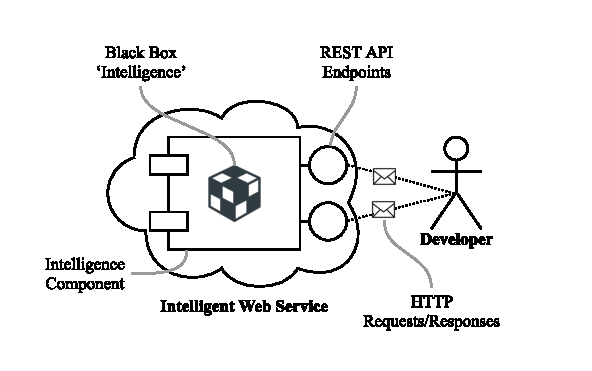
\includegraphics{cloud-intelliegnce-service}
\end{figure}

 
The general workflow of a \gls{cis} is  simple: a developer accesses a \gls{cis} component via \glsac{rest}/\glsac{soap} \gls{api}(s). For their given input, they receive an intelligent-like response typically serialised as \glsac{json}/\glsac{xml}. We note the intelligence component masks its `intelligence' through a black-box: in recent years, there is a rise in providing human-level intelligence via crowdsourcing Internet marketplaces such as Amazon Mechanical Turk~\citepweb{MTurk:Home} or ScaleAPI~\citepweb{ScaleAPI:Home}. Thus, a \gls{cis} may be powered by varying degrees of intelligence: human intelligence, machine learning, data mining or even intelligence by brute-force.

While there are different types of \glspl{cis} evident (such as OCR transcription, text-to-speech and speech-to-text, object categorisation, object comparison, natural language processing etc.), we scope the work investigated in this study to \glspl{cvcis}~\citepweb{GoogleCloud:Home,Azure:Home,AWS:Home,Pixlab:Home,IBM:Home,Cloudsight:Home,Clarifai:Home,DeepAI:Home,Imagaa:Home,Talkwaler:Home,Kairos:Home,Cognitec:Home,Affectiva:Home}. The ubiquity of \glspl{cvcis} is exemplified through evermore growing applications that use these \glspl{api}: aiding the vision-impaired \citep{Reis:2018cp,daMotaSilveira:2017vp}, accounting  \citep{Marshall:2018uj}, data analytics \citep{Iyengar:2017fb}, and student education \citep{Dibia:2017iy}. Moreover, we refer to its growing adoption in developer circles within \cref{fig:introduction:stackoverflow-trends}.

\section{Research Motivation}%: The Nondeterministic Impact to Quality}
\label{sec:introduction:motivation}

\todo{This section describes deterministic mindset clashing against probabilistic behaviour}

\todo{MA: It is useful to highlight the takeaways of each paragraph - e.g. probabilistic nature of ML, Choosing a threshold problem, lack of understanding of how ml works, documentation style of ml models. then at the end of the section, clearly state the problem/gap  considered}

\glspl{iws} are accessible through \glspl{api} consisting of `black box' intelligence (\cref{fig:introduction:cloud-intelliegnce-service}).\footnote{The `black box' refers to a system that transforms input (or stimulus)  to outputs (or response) without any understanding of the internal architecture by which this transformation occurs. This arises from a theory in the electronic sciences and adapted to wider applications since the 1950s--60s \citep{Ashby:1957db,Bunge:1963jm} to describe ``systems whose internal mechanisms are not fully open to inspection'' \citep{Ashby:1957db}. }
Data scientists produce \gls{ml} algorithms to make predictions in our datasets and discover patterns within them. These black boxes are inherently probabilistic and stochastic; there is little room for certainty in these results, as the insight is purely statistical and associational \citep{Pearl:2018uv} against its training dataset. 

Evermore applications are using \glspl{cvs} as demonstrated by ubiquitous examples: aiding the vision-impaired \citep{Reis:2018cp,daMotaSilveira:2017vp}, accounting  \citep{Marshall:2018uj}, data analytics \citep{Iyengar:2017fb}, and student education \citep{Dibia:2017iy}.
However, developers who build these applications do not need to treat their programs in a stochastic or probabilistic mindset manner, given a rule-driven mindset that computers make certain outcomes.
A \gls{cvs}, for example, may return the \textit{probability} that a particular object exists in an input images' pixels, and thus for a more certain (though not fully certain) distribution of overall confidence returned from the service, a developer must treat the problem stochastically by testing this case hundreds if not thousands of times to find a richer interpretation of the inference made. 

Unless a change in \gls{api} version occurs, educators teach application developers a deterministic mindset that an \gls{api} call returns the same outputs for the same inputs. As an example, consider simple arithmetic representations (e.g., $2+2=4$). The deterministic (rule-driven) mindset suggests that the result will \textit{always} be 4. However, the non-deterministic (data-driven) mindset suggests that results are probable: target output (\textit{exactly} 4) and the output inferred (\textit{a likelihood of} 4) matches as a probable percentage (or as an error where it does not match).\footnote{\citet{Blake:1998vd} produces a multi-layer perceptron \glslong{nn} performing arithmetic representation.} Instead of an exact output, there is a \textit{probabilistic} result: $2+2$ \textit{may} equal 4 to a confidence of $n$. 

Developers must appreciate such a critical principle of \gls{ml} software when building quality \gls{ai}-first applications, particularly reliability. The external quality of such software needs to consider reliability in the case of thresholding confidence values, that is whether the inference has an appropriate level of confidence to justify a predicted (and reliable) result to end-users. Selecting this confidence threshold is non-trivial; a \gls{ml} course from Google suggests that ``it is tempting to assume that [a] classification threshold should always be 0.5, but thresholds are problem-dependent, and are therefore values that you must tune.''~\citepweb{GoogleClassifcation:Thresholding}. Approaches to turning these values are considered for data scientists, but are not yet well-understood for application developers with little appreciation of the nuances of \gls{ml}. Similarly, developers should consider the internal quality of building \gls{ai}-first software. Reliable \gls{api} usability and documentation advocate for the accuracy, consistency and completeness of \glspl{api} and their documentation~\citep{Piccioni:2013em,Robillard:2009uk} and providers should consider mismatches between a developer's conceptual knowledge of the \gls{api} its implementation~\citep{Ko:2011fb}. Unreliable \glspl{api} ultimately hinder developer performance and thus reduces productivity. \Cref{ssec:introduction:motivation:scenario} provides two motivating scenarios describing these concerns in greater detail.
%
%% TODO: Copied from ml inconsistency paper
%\subsection{The Impact on Software Quality}
%\label{ssec:introduction:motivation:impact}
%
%Do traditional techniques for documenting deterministic \glspl{api} apply to non-deterministic systems? As \glspl{api} reflect a set of design choices made by their providers intended for use by the developer, does the mindset between the machine learning architect and the novice programmer match? 
%
%Moreover, \gls{iws} \glspl{api} are inherently non-deterministic in nature, but 
%In order to fully understand this problem, there are multiple dimensions one must consider: the impact of software quality; the fact that these systems underneath are probabilistic and are stochastic; the cognitive biases of determinism in developers; the issue of consistency in \gls{api} usage. While existing literature does extensively explore software quality and \gls{api} usability, these studies have only had emphasis on deterministic systems and thus little work to date has investigated such factors on probabilistic systems that make up the core of \glspl{cvs}. We explore more of these facets in the motivating scenarios below.

\subsection{Motivating Scenarios}
\label{ssec:introduction:motivation:scenario}

\todo{Could move this into the appendix to keep introduction chapter tighter}

\todo{JG: or could use one of these at start of section 1.2 to help clarify/motivate...}

\todo{yes too long in this chapter - use one, simplify a bit. Could put other one in appendix... }

\todo{MA: i guess the discussion related to Table1.3 and Table1.4 could be moved to 1.2 as one of the challenges}
\todo{MA: after reading the section, it looks like you could move it before 1.2}

The market for \glspl{iws} is increasing (\cref{fig:introduction:ai-products}) and as is developer uptake and enthusiasm in the software engineering community (\cref{fig:introduction:stackoverflow-trends}). However, the impact to software quality (internal and external) due to a mismatch of the application developer's deterministic  mindset and the service provider's nondeterministic mindset is of concern.

To illustrate the context of use, we present the two scenarios of varying risk: (i)~a fictional software developer, named Tom, who wishes to develop an inherently low-risk photo detection application for his friends and family; and (ii) a high-risk cancer \gls{cdss} that uses patient scans to recommend if surgeons should send their patients to surgery. Both describe scenarios where \gls{ai}-first components has substantiative impact to end-users when the software engineers developing with them misunderstand the nuances of \gls{ml}, ultimately adversely affecting external quality. Moreover, due to lack of comprehension, this hinders developer experience, productivity, and understanding/appreciation of \gls{ai}-based components.
  
\subsubsection{Motivating Scenario I: Tom's \textit{PhotoSharer} App}
\label{ssec:introduction:motivation:scenario:pam}

Tom wants to develop a social media photo-sharing app on iOS and Android, \textit{PhotoSharer}, that analyses photos taken on smartphones. Tom wants the app to categorise photos into scenes (e.g., day vs. night, landscape vs. indoors), generate brief descriptions of each photo, and catalogue photos of his friends and common objects (e.g., photos with his Border Collie dog, photos taken on a beach on a sunny day with his partner). His app will shares this analysed photo intelligence with his friends on a social-media platform, where his friends can search and view the photos.

Instead of building a computer vision engine from scratch, which takes too much time and effort, Tom thinks he can achieve this using one of the common \glspl{cvs}. Tom comes from a typical software engineering background and has insufficient knowledge of key computer vision terminology and no understanding of its underlying techniques. However, inspired by easily accessible cloud \glspl{api} that offer computer vision analysis, he chooses to use these. Built upon his experience of using other similar cloud services, he decides on one of the \gls{cvs} \glspl{api}, and expects a static result always and consistency between similar \glspl{api}. Analogously, when Tom invokes the iOS Swift substring method \texttt{"doggy".prefix(3)}, he expects it to be consistent with the Android Java equivalent \texttt{"doggy".substring(0, 2)}. Consistent, here, means two things: (i) that calling \texttt{substring} or \texttt{prefix} on \texttt{`dog'} will \textit{always} return in the same way every time he invokes the method; and (ii) that the result is \textit{always} \texttt{`dog'} regardless of the programming language or string library used, given the deterministic nature of the `substring' construct (i.e., results for substring are \gls{api}-agnostic). 

\begin{table}[th!]
  \centering
  \caption[Varying confidence changes over time between 3 CV APIs]{First six responses of image analysis for a Border Collie sent to three computer vision \gls{cis} \glspl{api} providers five months apart. The specificity (to 3 s.f.) and vocabulary of each label in the response varies between all services, and---except for Provider B---changes over time. Any confidence changes greater than 1 per cent are highlighted in red.}
  \label{tab:introduction:motivation:scenario:pam:confchanges}
  \begin{tabular}{l|c|c|c|c|c|c}
    \toprule
    \multirow{2}{*}{\bfseries Label} &
    \multicolumn{2}{c}{\bfseries Provider A} &
    \multicolumn{2}{c}{\bfseries Provider B} &
    \multicolumn{2}{c}{\bfseries Provider C} \\
    &
    Aug 2018 & Jan 2019 &
    Aug 2018 & Jan 2019 &
    Aug 2018 & Jan 2019 \\
    \midrule
    Dog             & 0.990 & \textcolor{red}{0.986} & 0.999 & 0.999 & 0.992 & \textcolor{red}{0.970} \\
    Dog Like Mammal & 0.960 & 0.962 & -     & -     & -     & -     \\
    Dog Breed       & 0.940 & 0.943 & -     & -     & -     & -     \\
    Border Collie   & 0.850 & 0.852 & -     & -     & -     & -     \\
    Dog Breed Group & 0.810	& 0.811 & -     & -     & -     & -     \\
    Carnivoran      & 0.810 & \textcolor{red}{0.680} & -     & -     & -     & -     \\
    Black           & -     & -     & 0.992 & 0.992 & -     & -     \\
    Indoor          & -     & -     & 0.965 & 0.965 & -     & -     \\
    Standing        & -     & -     & 0.792 & 0.792 & -     & -     \\
    Mammal          & -     & -     & 0.929 & 0.929 & 0.992 & \textcolor{red}{0.970} \\
    Animal          & -     & -     & 0.932 & 0.932 & 0.992 & \textcolor{red}{0.970} \\
    Canine          & -     & -     & -     & -     & 0.992 & \textcolor{red}{0.970} \\
    Collie          & -     & -     & -     & -     & 0.992 & \textcolor{red}{0.970} \\
    Pet             & -     & -     & -     & -     & 0.992 & \textcolor{red}{0.970} \\
    \bottomrule
  \end{tabular}
\end{table}

More concretely, in \cref{tab:introduction:motivation:scenario:pam:confchanges}, we illustrate how three (anonymised) \gls{cvs} providers fail to provide similar consistency to that of the substring example above. If Tom uploads a photo of a border collie\footnote{The image used for these results is \url{https://www.akc.org/dog-breeds/border-collie/}.} to three different providers in August 2018 and January 2019, he would find that each provider is different in both the vocabulary used between. The confidence values and labels within the \textit{same} provider varies within a matter of five months. The evolution of the confidence changes is not explicitly documented by the providers (i.e., when the models change) nor do they document what confidence means. Service providers use a tautological nature when defining what the confidence confidence values are (as presented in the \gls{api} documentation) provides no insight for Tom to understand why there was a change in confidence, which we show in \cref{tab:introduction:motivation:scenario:pam:tautological}, unless he \textit{knows} that the underlying models change with them. Furthemore, they do not provide detailed understanding on how to select a threshold cut-off for a confidence value. Therefore, he's left with no understanding on how best to tune for image classification in this instance. The deterministic problem of a substring compared to the nondeterministic nature of the \gls{iws} is, therefore, non-trivial.

\begin{table}[hbt]
  \centering
  \caption[Tautological definitions of confidence found in API documentation]{Tautological definitions of `confidence' found in the \gls{api} documentation of three common \gls{cvcis} providers.}
  \label{tab:introduction:motivation:scenario:pam:tautological}
  \begin{tabular}{l|p{0.8\linewidth}}
    \toprule
    \bfseries \gls{api} Provider &
    \bfseries Definition(s) of Confidence \\
    \midrule
    Provider A &
      \itshape  
      ``Score is the confidence score, which ranges from 0 (no confidence) to 1 (very high confidence).''
      \upshape
      \citepweb{Google:ConfidenceScore_DocsLabel}
      \bigskip
      
      \itshape  
      ``Deprecated. Use score instead. The accuracy of the entity detection in an image. For example, for an image in which the `Eiffel Tower' entity is detected, this field represents the confidence that there is a tower in the query image. Range [0, 1].'' 
      \upshape
      \citepweb{Google:ConfidenceScore_DotNet} 
      \bigskip
      
      \itshape  
      ``The overall score of the result. Range [0, 1]''
      \upshape
      \citepweb{Google:ConfidenceScore_DotNet} 
      \bigskip
    \\ 
    Provider B &
      \itshape  
        ``Confidence score, between 0 and 1... if there insufficient confidence in the ability to produce a caption, the tags maybe [sic] the only information available to the caller.''
      \upshape
      \citepweb{Azure:ConfidenceScore_HowToCall}
      \bigskip
      
      \itshape  
        ``The level of confidence the service has in the caption.''
      \upshape
      \citepweb{Azure:ConfidenceScore_JavaDocs}    
      \bigskip
    \\
    Provider C &
      \itshape  
        ``The response shows that the operation detected five labels (that is, beacon, building, lighthouse, rock, and sea). Each label has an associated level of confidence. For example, the detection algorithm is 98.4629\% confident that the image contains a building.''
      \upshape
      \citepweb{AWS:ConfidenceScore_DetectLabel}
      \bigskip
      
      \itshape  
        ``[Provider C] also provide[s] a percentage score for how much confidence [Provider C] has in the accuracy of each detected label.''
      \upshape
      \citepweb{AWS:ConfidenceScore_DetectObjScene}
    \\
    \bottomrule
  \end{tabular}
\end{table}


To make an assessment of these \glspl{api}, he tries his best to read through the documentation of different \gls{cvs} \glspl{api}, but he has no guiding framework to help him choose the right one. A number of questions come to mind:

\begin{itemize}
  \item What does `confidence' mean?%ICSME(?)
  \item Which confidence is acceptable in this scenario?%ICSE-Demo
  \item Are these \glspl{api} consistent in how they respond?%ICSME
  \item Are the responses in \glspl{api} static and deterministic?%ICSME
  \item Would a combination of multiple \gls{cvs} \glspl{api} improve the response?%ICWE
  \item How does he know when there is a defect in the response? How can he report it?%ICSE
  \item How does he know what labels the \gls{api} knows, and what labels it doesn't?%ICSE
  \item How does it describe his photos and detect the faces?%ICSE
  \item Does he understand that the \gls{api} uses a machine learnt model? Does he know what a \gls{ml} model is?%ICSE
  \item Does he know when models update? What is the release cycle?%ASE
\end{itemize}

Although Tom generally anticipates these \glspl{cvs} to not be perfect, he has no prior benchmark to guide him on what to expect. The imperfections appear to be low-risk, but may become socially awkward when in use; for instance, if Tom's friends have low self-esteem and use the app, they may be sensitive to the app not identifying them or mislabelling them. Privacy issues come into play especially if certain friends have access to certain photos that they are (supposedly) in; e.g., photos from a holiday with Tom and his partner, however if the \gls{api} identifies Tom's partner as a work colleague, Tom's partner's privacy is at risk.

Therefore, the level of risk and the determination of what constitutes an `error' is dependent on the situation. In the following example, an error caused by the service may be more dangerous.

% Motiviating Example 2: Google Cancer Detect API...

\subsubsection{Motivating Scenario II: Cancer Detection \gls{cdss}}
\label{ssec:introduction:motivation:scenario:cancer}

Recent studies in the oncology domain have used deep-learning \glspl{cnn} to detect \glspl{roi} in image scans of tissue (e.g., \citep{Liu:2018fa,Haenssle:2018bz,EhteshamiBejnordi:2017kq}), flagging these regions for doctors to review. Trials of such algorithms have been able to accurately detect cancer at higher rates than humans, and thus incorporating such capabilities into a \gls{cdss} is closer within reach.  Studies have suggested these systems may erode a practitioner's independent decision-making \citep{Jaspers:2011hy,Chambers:1991uh} due to over-reliance; therefore the risks in developing \glspl{cdss} powered by \glspl{iws} become paramount.

In \cref{fig:introduction:motivation:scenario:cancer} we present a context diagram for a fictional \gls{cdss} named \textit{CancerAssist}. A team of busy pathologists utilise CancerAssist to review patient lymph node scans and discuss and recommend, on consensus, if the patient requires an operation. When the team makes a consensus, the lead pathologist enters the verdict into CancerAssist---running passively in the background---to ensure there is no oversight in the team's discussions. When a conflict exists between the team's verdict and CancerAssist's verdict, the system produces the scan with \glspl{roi} it thinks the team should review. Where the team overrides the output of CancerAssist, this reinforces CancerAssist's internal model as a \gls{hitl} learning process.

\begin{figure}[th]
\centering
  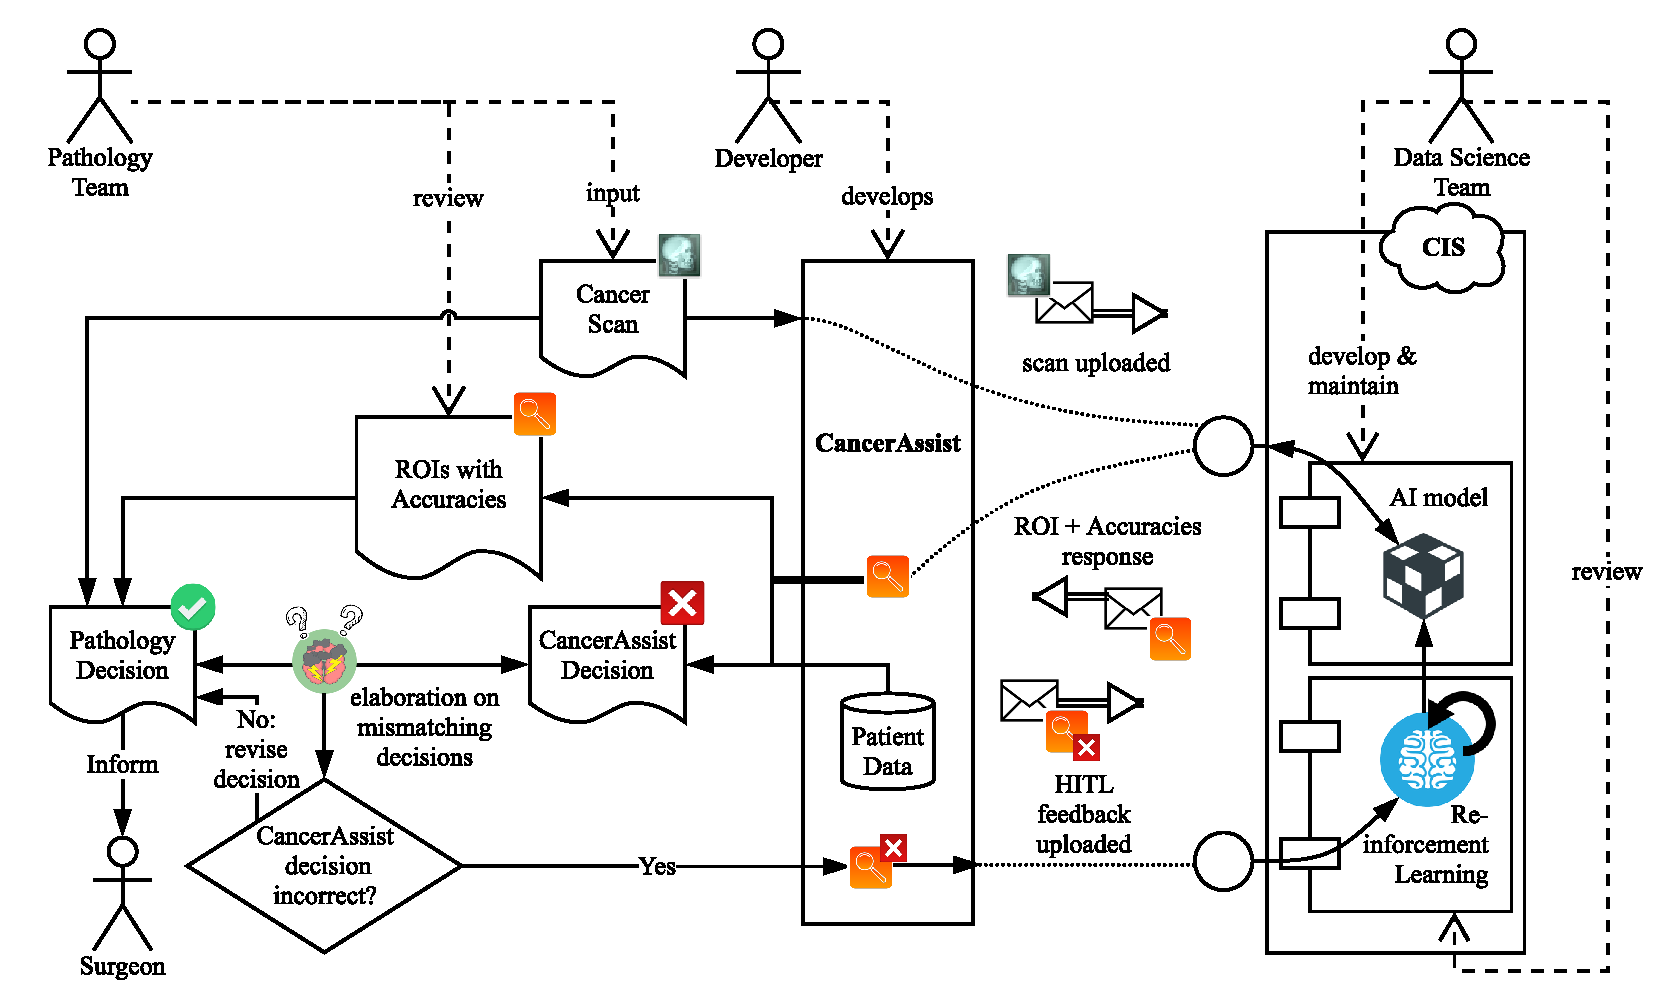
\includegraphics[width=0.85\linewidth]{cancer-assist}
  \caption[CancerAssist Context Diagram]{CancerAssist Context Diagram. \textit{\textbf{Key:} Red Arrows~=~Scan Input; Yellow Arrows~=~Decision Output; Blue Arrows~=~\gls{hitl} Feedback Input.}}
  \label{fig:introduction:motivation:scenario:cancer}
\end{figure}

Powering CancerAssist is Google AI's Lymph Node Assistant (LYNA) \citep{Liu:2018fa}, a \gls{cnn} based on the Inception-v3 model \citep{Szegedy:2016ws,Krizhevsky:2012wl}. To provide intelligence to CancerAssist, the development team decide to host LYNA as an \gls{iws} using a cloud-based \gls{paas} solution. Thus, CancerAssist provides \gls{api} endpoints integrated with patient data and medical history, which produces the verdict. In the case of a positive verdict, CancerAssist highlights the relevant \glspl{roi} found are with their respective bounding boxes and their respective cancer detection accuracies.

The developer of CancerAssist has no interaction with the Data Science team maintaining the LYNA \gls{iws}. As a result, they are unaware when updates to the model occur, nor do they know what training data they provide to test their system. The default assumptions are that the training data used to power the intelligence is near-perfect for universal situations; i.e., the algorithm chosen is the correct one for every assessable ontology tests in the given use case of CancerAssist. Thus, unlike deterministic systems---where the developer can manually test and validate the outcomes of the \glspl{api}---this is impossible for non-deterministic systems such as CancerAssist and its underlying \gls{iws}. The ramifications of not being able to test such a system and putting it out into production may prove fatal to patients.

Certain questions in the production of CancerAssist and its use of an \gls{iws} may come into mind:

\begin{itemize}%ASE
  \item When is the model updated and how do the \gls{iws} team communicate these updates?
  \item What benchmark test set of data ensures that the changed model doesn't affect other results?
  \item Are assumptions made by the \gls{iws} team who train the model correct?
\end{itemize}

Thus, to improve communication between developers and \gls{iws} providers, developers require enhanced documentation, additional metadata, and guidance tooling. 

%While developers are expected to use these services as they would any other traditional software component, the marketed promise is that such services are forever-learning and, therefore, `improve' in their accuracies and judgements. But what are the real-world consequences if this `black box' evolves with time and has materially substantiate impacts on both the software that is built on top of them, and (more importantly) the \textit{people} using that software? If the impact is substantial, the robustness of applications dependent on these services can have drastic effects, and---depending of the context of the application---the real-world damage it may do could be catastrophic. Should we consider this an `error' of the service?
%
%% Real world implications -- what is an error? (i.e., it depends on the application context)
%Whether or not it is an error is dependent on the context of the consuming application. For example, an educational mobile app designed to teach different dog breeds to children using a fine-grade visual categorisation service wouldn't be substantially erroneous should a Boston Terrier be misclassified as a French Bulldog---the \textit{ultimate effects} are not substantiate enough. However, consider a safety-critical application where an intelligent service performs facial recognition to identify a potential suspect in CCTV footage; evolution within the empowering \gls{iws} cannot be afforded, especially given the ethical and legal considerations if the wrong person is sentenced. If such risk is not mitigated, the accountability of these services must be considered~\citep{DoshiVelez:2017vm}.
%
%% Why is it happening? (DS land vs Eng. Land)
%Traditional software engineering principles advocate for software systems to be versioned upon substantial change, but unfortunately we find that the most prominent cloud vendors providing these intelligent services (Microsoft Azure, Google Cloud and Amazon Web Services) do not release new versioned endpoints of the APIs when the \textit{internal model} changes~\citep{Cummaudo:2019va}. In the context of computer vision, new labels may be introduced or dropped, entire ontologoies or specific training parameters may change, but we hypothesise that is not effectively communicated to developers. Broadly speaking, this can be attributed to a dichotomy of release cycles from the data science and software engineering communities: the data science iterations and work by which new models are trained and released runs at a faster cycle than the maintenance cycle of traditional software engineering. Thus we see cloud vendors integrating model changes without the \textit{need} to update the \gls{api} version unless substantial code or schema changes are also introduced---the nuance changes in the internal model does not warrant a shift in the \gls{api} itself, and therefore the version shift in a new model does not always propagate to a version shift in the \gls{api} endpoint.
%
%% Versioning alone is not enough!!
%Currently, it is impossible to invoke requests specific to a particular model that was trained at a particular date in time, and therefore developers need to consider how evolutionary changes of the services may impact their solutions \textit{in production}. Again, whether there is any noticeable behavioural changes from these changes is dependent on the context of the problem domain---unless developers benchmark these changes against their own domain-specific dataset and frequently check their selected service against such a dataset, there is no way of knowing if substantive errors have been introduced. 
%
%Given that such substantiative \gls{se} principles on versioning, quality and robustness are under-investigated within the context of \glspl{iws}, we aim to explore guidance from the \gls{se} literature to investigate what aspects in the development lifecyle could aide in mitigating these issues when developing using \gls{ai}-based components. The following section explains the research outcomes resolving from this thesis.
\section{Research Outcomes}
\label{sec:introduction:hypohtesis}

\itshape
In this thesis, we explore the probabilistic ripple-effect with relation to the development usability of `intelligent' \glspl{api}; specifically, we contextualise within computer vision \glspl{cis}. Our anchoring perspective is software quality---specifically, validation and verification---within such systems and what best practices within the field of software engineering can be applied to assist in operationalisation such systems.
\upshape

The goals of this study aim to provide a snapshot of current developer best practices towards the usage of \glspl{cis} to provide a guiding framework and recommendations for software developers and \glspl{cis} providers alike. Based on the motivating case studies in \cref{sec:introduction:motivation}, we articulate three Research Hypotheses (RH1--3) below.

\begin{titled-frame}{\underline{RH1}: \textit{Existing \glspl{cis} present insufficient \gls{api} documentation for general use.} }
\vspace{-12pt}
\paragraph{Research Hypothesis}
\gls{api} documentation of intelligent services are inadequate and insufficient given the disparity of mindsets between the software engineer and data scientist. Chiefly, software engineers---all with varied experience of using AI-based development tooling, if any---may have very limited general understanding of the `magic' that occurs behind these probabilistic `intelligent' \glspl{api}. We do not know what key aspects of the documentation matter to them, nor what they do or do not understand of the existing documentation.

\paragraph{Research Goal}
To improve the documentation of existing \gls{cis} providers, specifically of computer vision \glspl{api}.

\paragraph{Research Questions}
\begin{enumerate}[label=\textbf{RQ1.\arabic*.}, ref=RQ1.\arabic*, leftmargin=3.5\parindent, rightmargin=1\parindent]
  \item What practices are in use for intelligent services' \gls{api} documentation?
  \label{rqs:apidoc:what-is-in-use}
  
  \item How do developers currently understand and interpret the documentation given a lack of formal training in artificial intelligence? That is, what do they understand and not understand , and what key aspects of the \gls{api} documentation matter do developers as they see it?
  \label{rqs:apidoc:how-do-devs-understand-it}
  
  \item What additional information or attributes need to be included in the \gls{api} documentation?
  \label{rqs:apidoc:what-additional-information-needed}
\end{enumerate}

\paragraph{Research Contribution} An intelligent service \gls{api} documentation quality assessment framework to evaluate how well the service has been documented for software engineers to use.

\paragraph{Research Method}

Problem identification and discovery to validate our hypothesis in the \textit{general context} of \gls{api} usage will begin with a literature review to help inform what prior works have been done in the \gls{api} documentation space. We will follow this with repository and question mining, i.e., searching on developer communities such as Quora, Stack Overflow, and GitHub Issues to find out what developers complain about and mine this knowledge into a framework.

We then will conduct an internal pre-controlled survey within our research group (we refer to as the `pilot' survey study) and will use findings from the literature review and mining to help inform us of the kinds of questions to ask. 

Findings from the pilot survey to help inform a wider structured survey and unstructured interview, where we will recruit external software engineers in industry through contacts of our research group. A quantitative (survey) and qualitative (interview) analysis will help begin to shape our research outcome of an API documentation quality assessment framework and help stabilise a general understanding of how developers use the existing \glspl{api}.
\end{titled-frame}

\begin{titled-frame}{\underline{RH2}: \textit{Existing \glspl{cis} present insufficient metadata for context-specificity.} }
\vspace{-12pt}
\paragraph{Research Hypothesis}
Intelligent service \glspl{api} respond with insufficient information for developers to operationalise the service into a business-driven application and, thus, additional metadata is needed to assist developers. Such metadata is likely to be added to the response objects of the \gls{api}.

\paragraph{Research Goal}
To improve the quality of \textit{context-specific response data} from the \gls{api} endpoints of intelligent services.

\paragraph{Research Questions}
\begin{enumerate}[label=\textbf{RQ2.\arabic*.}, ref=RQ2.\arabic*, leftmargin=3.5\parindent, rightmargin=1\parindent]
  \item What are current problems due to lack of return metadata?
  \label{rqs:metadata:what-problems-due-to-lack-of-metadata}
  
  \item What kind of metadata do developers want? Why do they want this metadata?
  \label{rqs:metadata:what-metadata-do-devs-want-and-why}
  
  \item How does the metadata assist developers in developing applications that use intelligent services of varying contexts?
  \label{rqs:metadata:how-does-metadata-assist-devs}
\end{enumerate}

\paragraph{Research Contributions} A list of metadata key-value-pairs that assist developers in using these \glspl{api} during the development of software that consume these services. In essence, improvements to the framework of Research Outcome 1: ``\textit{An intelligent service \gls{api} documentation \underline{\upshape and metadata} quality assessment framework}''.

\paragraph{Research Method} To confirm findings of the method within RH1 is genuine, we shift from reviewing the documentation from a general stance to a specialised (context-specific) stance in the use of these \glspl{api}.

Thus, we will use context-specific action research to develop basic `prototypes' of varying contexts to help identify where any potential gaps are in the findings of RH1.
To validate the findings of developer opinion in the surveys and interviews of RH1 are indeed genuine, this helps ensure that there is nothing missing by adding in further context to such opinions.
\end{titled-frame}

\begin{titled-frame}{\underline{RH3}: \textit{RH1 and RH2 improve quality,  productivity or developer informativeness.} }
\vspace{-12pt}
\paragraph{Research Hypothesis}
The implication of hypotheses 1 and 2 suggest that improving both the documentation and providing further metadata will improve product quality (internal or external), and/or developer productivity and/or developer education in developing software with intelligent components.

\paragraph{Research Goal}
 To confirm if improvements to \gls{api} documentation and response metadata  are reflected as improvements to product quality, developer productivity and/or developer education.
 
 \paragraph{Research Questions}
\begin{enumerate}[label=\textbf{RQ3.\arabic*.}, ref=RQ3.\arabic*, leftmargin=3.5\parindent, rightmargin=1\parindent]
  \item  What metrics are improved when the intelligent service documentation or metadata is improved?
  \label{rqs:implications:what-metrics-improve}
  
  \item With respect to \ref{rqs:implications:what-metrics-improve}, the three aspects are explored:

  \begin{enumerate}
  \item Are improvements reflected in product quality (i.e., improve avoiding common pitfalls; external quality)?
  \item Are improvements reflected in developer productivity (e.g., faster, better, fewer bugs; internal quality)?
  \item Are improvements reflected as a subjective `feel-good' factor for the developer (e.g., is the developer better informed or more confidence in what they do)?
  \end{enumerate}
  \label{rqs:implications:aspects}  
\end{enumerate}

\paragraph{Research Contribution}
A concrete sample solution or framework that improves such metrics, thereby confirming that our documentation and metadata quality assessment framework improves these facets.

\paragraph{Research Method}

To confirm that the framework is valid, we will provide a fictitious \gls{api} that is documented with the additional metadata and information organised using our framework.

We then ask 20 developers to complete five tasks under an observational, comparative controlled study, 10 of which will (a) develop with the new framework, and the other 10 will (b) develop with the as-is/existing documentation. From this, we compare if the framework makes improvements by capturing metrics and recording the observational sessions for qualitative and quantitative analysis.
\end{titled-frame}

Ultimately, we seek to understand the conceptual understanding of software engineers who operationalise stochastic and probabilistic systems, and furthermore understand knowledge representation with these systems' \gls{api} documentation. Our motivation is to provide insight into current practices and compare the best practices with actual practise. We strive for this to  provide developers with a guiding framework on how to best operationalise these systems via the form of some checklist or tool they can use to ensure optimal software quality.

It is anticipated that the findings from this study in the computer vision \glspl{cis} space will be generalisable to other areas, such as time-series information, natural language processing and others.

%  Paper 2:
%* RQ1. How do software engineers evaluate (knowledge representation) machine learning APIs for use in an application?
%   * Motivation: to provide insights into the current practice
%   * Method: Survey
%* RQ2. Do software engineers follow best practices when evaluating machine learning APIs?
%   * Motivation: to compare best practice with actual practice
%   * Survey
%\section{Methodology}
%\label{sec:introduction:methodology}
%

\section{Contributions}
\section{Thesis Organisation}
\label{sec:introduction:organisation}

We organise the thesis into four parts. \textbf{\Cref{part:preface}~(\textit{The Preface})} includes introductory, background, and methodology chapters. This is a \textit{PhD by Publication}, and \textbf{\cref{part:publications}~(\textit{Publications})} comprises of eight publications resulting from this work over \cref{ch:icsme2019,ch:tse2020,ch:icse2020,ch:fse-demo2020,ch:fse2020,ch:icwe2019,ch:semotion2021,ch:caise2021}; publications are included verbatim except for terminology and formatting changes to better fit the suitability of a coherent thesis. \textbf{\Cref{part:postface}~(\textit{The Postface})} includes the conclusion and future works chapter, as well as a list of academic studies and online artefacts referenced throughout the thesis. \textbf{\Cref{part:appendices}~(\textit{Appendices})} includes all supplementary material, including mandatory authorship statements and ethics approval. Details of each chapter following this introductory chapter are provided in the following section.

\subsection[Part I: Preface]{\Cref{part:preface}: Preface}

\subsubsection[Chapter 2: Background]{\cref{ch:background}: Background} This chapter provides an overview of prior studies broadly around the development, usage, and nature of \glspl{iws}. We use three perspectives to describe prior work; that of of software quality (particularly, reliability), probabilistic and non-deterministic systems, and explanation and communication theory.

\subsubsection[Chapter 3: Research Methodology]{\cref{ch:research-methodology}: Research Methodology} This chapter provides a summative review of research methods and philosophical stances relevant to software engineering. We illustrate that the methods used within our publications are sound via an analysis of the methodologies used in seminal works referenced in this thesis.

\subsection[Part II: Publications]{\Cref{part:publications}: Publications}

\subsubsection[Chapter 4: Exploring the nature of CVSs]{\cref{ch:icsme2019}: Exploring the nature of \glspl{cvs}} This chapter was presented at the \textbf{2019 International Conference on Software Maintenance and Evolution~(ICSME)}~\citep{Cummaudo:2019icsme}. We describe an 11-month longitudinal study assessing the behavioural (run-time) issues of three popular \glspl{cvs}: Google Cloud Vision~\citepweb{GoogleCloud:Home}, Amazon Rekognition~\citepweb{AWS:Home} and Azure Computer Vision~\citepweb{Azure:Home}. By using three different data sets---two of which we curate as additional contributions---we demonstrate how the services are inconsistent amongst each other and within themselves. This study answers \ref{rq:nature}: Despite presenting conceptually-similar functionality, each service behaves and produces slightly varied (inconsistent) results and demonstrates non-deterministic runtime behaviour. We discuss potential evolution risks to consumers of such services as the services provide non-static outputs for the same inputs, thereby having significant impact to the robustness of consuming applications. Further details in the study include a brief assessment into the lack of sufficient detail of these concerns in their documentation.

\subsubsection[Chapter 5: Understanding developer struggles when using CVSs]{\cref{ch:icse2020}: Understanding developer struggles when using \glspl{cvs}} This chapter was presented at the \textbf{2020 International Conference on Software Engineering~(ICSE)}~\citep{Cummaudo:2020icse}. We conduct a mining study of 1,425 \glslong{so} questions that provide indications of the types frustrations that developers face when integrating \glspl{cvs} into their applications. To gather what their pain-points are, we use two classification taxonomies that also utilise \glslong{so} to understand generalised and documentation-specific pain-points in mature software engineering domains. This study answers \ref{rq:devs} in detail and provides a validation to our motivation of \ref{rq:docs}: we validate that the \textit{completeness} of current \gls{cvs} \gls{api} documentation is a main concern for developers and there is insufficient explanation into the errors and limitations of the service. We find that the documentation does not adequately cover all aspects of the technical domain. In terms of integrating with the service, developers struggle most with simple errors and ways in which to use the \glspl{api}; this is in stark contrast to mature software domains. Our interpretation is that developers fail to understand the \gls{iws} lifecycle and the `whole' system that wraps such services. We also interpret that developers have a shallower understanding of the core issues within \glspl{cvs} (likely due to the nuances of \gls{ml} as suggested in a discussion in the paper), which warrants an avenue for future work in software engineering education.

\afterpage{
\begin{landscape}
\begin{table}
  \centering
  \caption[List of publications resulting from this thesis]{List of publications resulting from this thesis, separated by phenomena exploration (above) and solution design (below).}
  \label{tab:introduction:structure:list-of-pubs}
  \tablefitlandscape{0.8}{\begin{tabular}{rp{0.335\linewidth}ccc|cc}
    \toprule
    \textbf{Ref.} &
    \textbf{Venue} &
    \textbf{Acronym} &
    \textbf{Rank\tablefootnote{Measured as at Jan 2020 using CORE Conference (\url{http://www.core.edu.au/conference-portal}) and Scimago Rankings (\url{https://scimagojr.com/}).}} &
    \textbf{Published\tablefootnote{Date of publication, if applicable.}} &
    \textbf{Chapter} &
    \textbf{RQs}\\
    \midrule
    
    % ICSME
    \citep{Cummaudo:2019icsme} &
    35\textsuperscript{th} International Conference on Software Maintenance and Evolution &
    ICSME &
    A &
    Sep 2019 &
    \cref{ch:icsme2019} &
    \ref{rq:nature} \\

    % ESEM
    \citep{Cummaudo:2019esem} &
    13\textsuperscript{th} International Symposium on Empirical Software Engineering and Measurement &
    ESEM &
    A &
    Sep 2019 &
    Excluded\tablefootnote{The extended version of this conference proceeding is provided in \citep{Cummaudo:2020tse}, \cref{ch:tse2020}.} &
    \ref{rq:docs:complete} \\
    
    % ICSE
    \citep{Cummaudo:2020icse}&
    42\textsuperscript{nd} International Conference on Software Engineering&
    ICSE &
    A* &
    Jun 2020&
    \cref{ch:icse2020}&
    \ref{rq:devs} \\
    
    % SEmotion
    \citep{Cummaudo:2021semotion}&
    6\textsuperscript{th} International Workshop on Emotion Awareness in Software Engineering\tablefootnote{An ICSE 2021 workshop.}&
    SEmotion&
    A* &
    \textit{In Press}&
    \cref{ch:semotion2021}&
    \ref{rq:devs:frustration}\\
    
    % CAiSE
    \citep{Graetsch:2021caise}&
    33\textsuperscript{rd} International Conference on Advanced Information Systems Engineering&
    CAiSE&
    A &
    \textit{In Review}&
    \cref{ch:caise2021}&
    \ref{rq:devs:frustration}\\
    
    \midrule
    
    % TSE
    \citep{Cummaudo:2020tse}&
    IEEE Transactions on Software Engineering & 
    TSE &  
    Q1&
    Dec 2020& 
    \cref{ch:tse2020} &
    \ref{rq:docs} \\
    
    % ICWE
    \citep{Ohtake:2019vi} & 
    13\textsuperscript{th} International Conference on Web Engineering&
    ICWE&
    B&
    Apr 2019 &
    \cref{ch:icwe2019} &
    \ref{rq:design} \\
     
    % FSE
    \citep{Cummaudo:2020fse}&
    28\textsuperscript{th} Joint European Software Engineering Conference and Symposium on the Foundations of Software Engineering&
    FSE&
    A*&
    Nov 2020 &
    \cref{ch:fse2020} &
    \ref{rq:design} \\

    % FSE(d)
    \citep{Cummaudo:2020fse-demo}&
    28\textsuperscript{th} Joint European Software Engineering Conference and Symposium on the Foundations of Software Engineering&
    FSE(d)\tablefootnote{We abbreviate this with an added `d' (for the demonstrations track) to distinguish this paper from our full FSE 2020 paper.} &
    A* &
    Nov 2020&
    \cref{ch:fse-demo2020} &    
    \ref{rq:design} \\

    \bottomrule
  \end{tabular}}  
\end{table}
\end{landscape}
}

\subsubsection[Chapter 6: Ranking CVS pain-points by frustration]{\cref{ch:semotion2021}: Ranking \gls{cvs} pain-points by frustration} This chapter has been published as a technical report pre-print on arXiv and an extended version was accepted as a paper at the \textbf{2021 International Workshop on Emotion Awareness in Software Engineering (SEmotion)}~\citep{Cummaudo:2021semotion}. In this work, we use our dataset consisting of the 1,425 Stack Overflow questions from \citep{Cummaudo:2020icse} to interpret the breakdown of emotions developers express per classification of pain-points conducted in \cref{ch:icse2020}. We find that the distribution of various emotions differ per question type, and developers are most frustrated when the expectations of a \gls{cvs} does not match the reality of what these services actually provide, shaping our answers for \ref{rq:devs:frustration} and thus \ref{rq:devs}.

\subsubsection[Chapter 7: Lessons in applying pre-trained models to Stack Overflow]{\cref{ch:caise2021}: Lessons in applying pre-trained models to Stack Overflow} This chapter is \textbf{in review} for the \textbf{2021 International Conference on Advanced Information Systems Engineering (CAiSE)}~\citep{Graetsch:2021caise}. This work presents a deeper investigation into the classification model used within \cref{ch:semotion2021} to better interpret the automation effort we conducted, thereby highlighting valuable lessons we learnt from performing this exercise. Specifically, we find that the classification model we used in this exercise presented substantial data imbalance, which presented unexpected results (namely, a high level of  \glslong{so} questions that showed the emotion, `love'). We identify how novel documentation tooling such as model cards \citep{Mitchell:2018in} or datasheets \citep{Gebru:2018wh} could have identified risks to our study earlier, and make suggestions needed into future documentation efforts. This work presents complementary  results to \ref{rq:docs} to help propose which documentation elements \gls{ml} models (and thus \glspl{iws}) should provide before diving `straight in'.

\subsubsection[Chapter 7: Investigating improvements to CVS API documentation]{\cref{ch:tse2020}: Investigating improvements to \gls{cvs} \gls{api} documentation} This chapter was accepted as a paper at the \textbf{2019 International Symposium on Empirical Software Engineering and Measurement~(ESEM)} \citep{Cummaudo:2020icse}. The extended version of this chapter will be published in an upcoming issue of the \textbf{IEEE Transactions on Software Engineering (TSE)}~\citep{Cummaudo:2020tse}, currently available as a preprint. To understand where to improve \gls{cvs} documentation, we first need to investigate \textit{what} makes a good \gls{api} document. This short paper initially answered one aspect of \ref{rq:docs:complete}: the research effort in academic literature to study various \gls{api} documentation artefacts. By conducting an \glslong{sms} resulting in 21 primary studies, we systematically develop a taxonomy that combines documentation artefacts studied in scattered work into a structured framework of 5 dimensions and 34 weighted categorisations. We then extend this work by triangulating the taxonomy with opinions from developers using a survey to assess the efficacy of these artefacts (thereby answering the second aspect of \ref{rq:docs:complete}). From this, we assess how well \gls{cvs} providers document their \glspl{api} via a heuristic validation of the taxonomy, using the three services from the ICSME publication to make recommendations where documentation should be more complete, thereby answering \ref{rq:docs:missing} (and thus \ref{rq:docs}).

\subsubsection[Chapter 8: Merging responses of multiple CVSs]{\cref{ch:icwe2019}: Merging responses of multiple \glspl{cvs}} This chapter was presented at the \textbf{2019 International Conference on Web Engineering~(ICWE)}~\citep{Ohtake:2019vi}. Early exploration of \glspl{cvs} showed that multiple services use vastly different ontologies for the same input. As an initial strategy to improve the reliability of these services, we explored if merging multiple responses using WordNet \citep{WordNetMiller1995} and a novel label merging algorithm based on the proportional representation approach used in political voting could make any improvements. While this approach resulted in a modest improvement to reliability, it did not consider to the evolution issues or developer pain-points we later identified.

\subsubsection[Chapter 9: Developing a CVS integration architecture]{\cref{ch:fse2020}: Developing a \gls{cvs} integration architecture} This chapter was presented at the \textbf{2020 Joint European Software Engineering Conference and Symposium on the Foundations of Software Engineering (ESEC/FSE)}~\citep{Cummaudo:2020fse}. Based on the findings, we propose a set of new service error codes for describing the empirically observed error conditions of \gls{iws} based on our findings in \cref{ch:icsme2019}. To achieve this, we propose a proxy server intermediary that lies between a client application and a \gls{iws}; the proxy server tactic is designed to return these error codes when substantial evolution occurs against a benchmark dataset that represents the application domain context. A technical evaluation of our implementation of this architecture identifies 1,054 cases of substantial evolution in confidence values and 2,461 cases of evolution in the response label sets when 331 images were sent to a \gls{cvs}. This study forms a key contribution to answer \ref{rq:design} and improve robustness of integrating conventional software components with \glspl{iws}.

\subsubsection[Chapter 10: Developing a confidence thresholding tool]{\cref{ch:fse-demo2020}: Developing a confidence thresholding tool} This chapter is an example implementation of the threshold tuner component discussed in \cref{ch:fse2020}, and was published under the tool demonstrations track of the \textbf{2020 Joint European Software Engineering Conference and Symposium on the Foundations of Software Engineering (ESEC/FSE)}~\citep{Cummaudo:2020fse-demo}. When integrating with a \gls{cvs}, developers need to select an appropriate confidence threshold suited to their use case and determine whether a decision should be made. An issue, however, is that these \glspl{cvs} are not calibrated to the specific problem-domain datasets and it is difficult for software developers to determine an appropriate confidence threshold on their problem domain. This tool presents a workflow and supporting tool for application developers to select decision thresholds suited to their domain that---unlike existing tooling---is designed to be used in pre-development, pre-release and production. This tooling forms part of a solution to \ref{rq:design} for developers to maintain robustness and reliability in their systems.

\subsection[Part III: Postface]{\Cref{part:postface}: Postface}

In \Cref{ch:conclusions}, we review the contributions made in this thesis and the relevance and significance to identifying and resolving key issues when application developers integrate with \glspl{cvs}. We evaluate these outcomes with reference to the research goals, and discuss threats to validity of the work. Lastly, we discuss the various avenues of research arising from this work. References from literature and a list of online artefacts are provided after this concluding chapter.

\subsection[Part IV: Appendices]{\Cref{part:appendices}: Appendices}

\Cref{ch:additional-materials} thru \cref{ch:ethics} are appendices. \Cref{ch:additional-materials} provides supplementary figures to the studies performed in this thesis. The source code for the reference architecture described in \cref{ch:fse2020} is reproduced in \cref{ch:reference-architecture-code}. The supplementary materials published with \cref{ch:tse2020} are reproduced in \cref{ch:tse-supplementary-materials}, which also describes the list of primary sources arising in the \glslong{sms} we conducted.
 We provide mandatory coauthor declaration forms describing the contribution breakdown for each publication within \cref{ch:authorship-statements}. \Cref{ch:ethics} contains copies of the ethics clearance for various studies within this thesis. 

\section{Research Contributions}
\label{sec:introduction:research-contributions}

The outcomes of answering the four primary research questions elaborated in \cref{sec:introduction:goals} shapes three primary contributions this thesis offers to software engineering knowledge:

\begin{enumerate}
  \item An \textbf{improved understanding in the landscape of \glspl{cvs}}, with respect to their runtime behaviour and evolutionary profiles. 
  \item A novel \textbf{service integration architecture} that helps developers with integrating their applications with \glspl{cvs}.
  \item A \textbf{key list of attributes that should be documented}, to assist \gls{cvs} providers to better document their services.
\end{enumerate}

In this section, we detail how each publication forms a coherent body of work and how each publication relates to the primary contributions made. After our exploratory analysis on the nature of \glspl{cvs} (\cref{ch:icsme2019}), we proposed two sets of recommendations targeted towards two stakeholders: (i) the service \textit{consumers} (i.e., application developers), and (ii) the service \textit{providers}. Our subsequent publications arose as a two-fold investigation to develop two strategies in which developers and providers can, respectively, (i) better integrate these intelligent components into their applications, and (ii) how these services can be better documented. These two contributions are \textit{disparate} and stem from the initial investigations to explore \gls{cvs} runtime and evolutionary behaviour (i.e., contribution 1); thus the publications relating to the second and third contributions should not be interpreted as subsequent works that `build' onto each other. To visualise how each of the studies fit in to our thesis narrative, a high-level overview representing the cohesiveness of our publications is provided in \cref{fig:introduction:structure:publications-overview}. Further, \cref{tab:introduction:structure:list-of-pubs} provides a tabulated form of the publications and research questions addressed within this thesis; for ease of reference, we refer to the publications in within this section in their abbreviated form as listed in \cref{tab:introduction:structure:list-of-pubs}.

\begin{figure}[t!]
  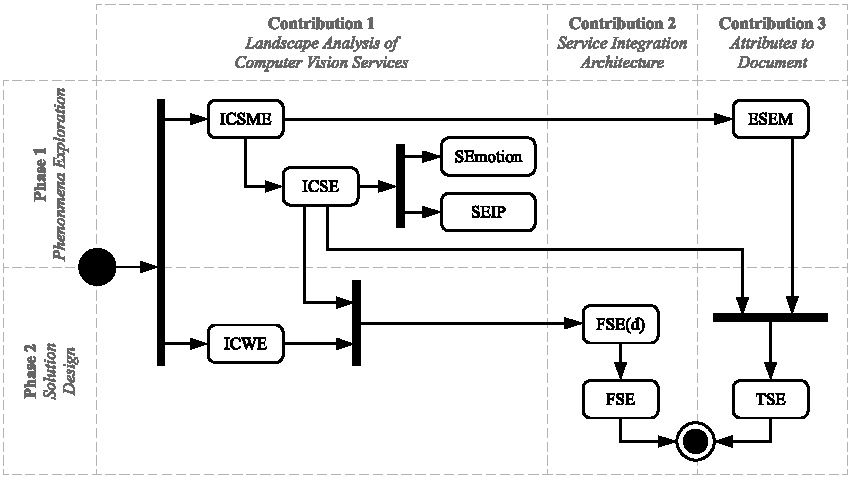
\includegraphics[width=\linewidth]{publications-overview}
  \caption[Overview publication coherency]{Activity diagram of the coherency of our publications, how our research was conducted, and relevant connections between publications. Our two-phase structure initial phenomena exploration and a proposed solutions to issues identified from the exploration. We map the contributions within each publication to the three primary contributions of the thesis. Acronyms of each publication are provided in \cref{tab:introduction:structure:list-of-pubs}.}
  \label{fig:introduction:structure:publications-overview}
\end{figure}

\subsection{Contribution 1: Landscape Analysis \& Preliminary Solutions}

The first two bodies of work in this paper are the ICSME and ICWE papers. These two works investigated a landscape analysis \glspl{cvs} from two perspectives: firstly, we conducted a longitudinal study to better understand the attributes associated with these services (ICSME)---particularly their evolution and behavioural profiles, and their potential impacts to software reliability---and tackled a preliminary solution facade to `merge' responses of the services together (ICWE). 

The ICSME paper confirmed our hypotheses that the services have a non-deterministic behavioural profile, and that the evolution occurring within the \gls{ml} models powering these services are not sufficiently communicated to software engineers. This therefore led to follow up investigation into how developers perceive these services to determine if they are frustrated due to this lack of communication. 

Our ICWE paper explored one aspect identified from the ICSME paper that we noticed: that different services use different vocabularies to describe semantically similar objects but in different ways (e.g., `border collie' vs. `collie'), despite offering functionally similar capabilities. We attempted to merge the response labels from these services using a proportional representation approach, and upon comparison with more naive merge approaches, we improved label-merge performance by an F-measure of 0.015. However, while this was an interesting outcome for a preliminary solution design, investigation from our following work suggested that standardising ontologies between service providers becomes challenging and normalising the entire ontological hierarchy of response labels would need to fall under the responsibility of a certain body (that does not exist). Further, we did not find sufficient evidence that developers would frequently switch between service providers. Therefore, we opted for a shielded relay architecture in our later design work.  

\subsection{Contribution 2: Improving Documentation Attributes}

As mentioned, our ICSME paper found that evolutionary and non-deterministic behavioural profile of are not adequately documented in pre-trained \gls{ml} model \gls{api} documentation. As developers learn, improve, and deepen their skills from such \gls{api} documentation, it is important that these aspects are clearly communicated. Unclear or poor documentation, therefore, has an adverse impact to productivity. Similarly, heightened emotions in the software development process (e.g., the \glslong{so} issues presenting with strong sentiment as shown in \cref{ch:semotion2021,ch:caise2021}) further results in deeper frustration with these services, and thus reduced productivity. Ultimately, productivity can be alleviated with improved service documentation.

A recommendation concluding from our ICSME study was that service providers should improve their documentation, however there lacked a strategy by which they could do this, and our hypotheses that developers were actually frustrated by this lack of communication was yet to be tested. This led to two follow-up further investigations as presented in our ICSE and ESEM papers.

One aspect of our ICSE paper was to confirm whether developers are actually frustrated with the service's limited \gls{api} documentation. By mining \glslong{so} posts with reference to documentation issues, we adopted a \citeyear{Aghajani:2019bo} documentation-related taxonomy by \citet{Aghajani:2018et} to classify posts, and found that 47.87\% of posts classified fell under the `completeness' dimension of \citeauthor{Aghajani:2018et}'s taxonomy. This interpretation, therefore, warranted the recommendation proposed in the ICSME paper to improve service documentation. 

However, though improvements to more complete documentation was justified from the ICSE paper, we needed to explore exactly \textit{what} makes a `complete' \gls{api} document. By conducting a \glslong{sms} resulting in 4,501 results, we curated 21 primary studies that outline the facets of \gls{api} documentation knowledge. From these studies, we distilled a documentation framework describing a prioritised order of the documentation assets \gls{api}'s should document that is described in our ESEM short paper. After receiving community feedback, we extended this short paper with a follow-up study submitted to TSE. By conducting a survey with developers, we assessed our \gls{api} documentation taxonomy's efficacy with practitioner opinions, thereby producing a weighted taxonomy against \textit{both} literature and developer sources. Lastly, we triangulated both weightings against a heuristic evaluation against common \gls{cvs} providers' documentation. This allowed us to deduce which specific areas in existing \gls{cvs} providers' \gls{api} documentation needed improvement, which was a primary contribution from our TSE article.

\subsection{Contribution 3: Service Integration Architecture}

Two recommendations from our ICSME study encouraged developers to test their applications with a representative ontology for their problem domain and to incorporate a specialised testing and monitoring techniques into their workflow. Strategies on \textit{how} to achieve this were explored in later studies.  Following a similar approach to our solution of improved \gls{api} documentation, we validated the substantiveness of our recommendations using our mining study of \glslong{so} (our ICSE paper) to help inform us of generalised issues developers face whilst integrating \glspl{cvs} into their applications. To achieve this, we used a \glslong{so} post classification taxonomy proposed by \citet{Beyer:2018fm} into seven categories, where 28.9\% and 20.37\% of posts asked issues regarding how to use the \gls{cvs} \gls{api} and conceptual issues behind \glspl{cvs}, respectively. Developers presented an insufficient understanding of the non-deterministic runtime behaviour, functional capability, and limitations of these services and are not aware of key computer vision terminology. When contrasted to more conventional domains such as mobile-app development, the spread of these issues vary substantially.

We proposed two technical solutions in our two FSE papers to help alleviate this issue. Firstly, our FSE demonstrations paper---FSE(d) for short---provides a workflow for developers to better select an appropriate confidence threshold, and thus decision boundary, calibrated for their particular use case. In our ESEC/FSE paper, we provide a reference architecture for developers to guard against the non-deterministic issues that may `leak' into their applications. This architecture tactic proposes a client-server intermediary proxy server, similar to the style proposed in our ICWE paper. However, unlike the ICWE paper that uses proportional representation approach to modify multiple sources, our FSE paper proposes a guarded relay, whereby a single service is used, and the proxy server maintains a lifecycle to monitor evolution issues identified in ICSME and should be benchmarked against the developer's dataset (i.e., against the particular application domain) as suggested in FSE(d). For robust component composition, this architecture tactic handles four key requirements: (i) it clearly defines erroneous conditions that occur when evolution occurs in \glspl{cvs}; (ii) it notifies of behavioural changes in the service; (iii) it monitors the service for change and substantial impact this may have to the client application; and (iv) is flexible enough to be implemented and adaptable to any client application or specific intelligent service to facilitate reuse. Both FSE papers serve as two primary contributions to \ref{rq:design}.

% RQ3.3 -- range is diff == existing strategies are not enough!